\documentclass[preprint,12pt,a4paper]{elsarticle}

\usepackage{amssymb}
\usepackage{amsmath}
\usepackage{graphicx}
\usepackage{booktabs}
\usepackage{hyperref}
\usepackage{listings}
\usepackage{xcolor}
\usepackage{tikz}
\usepackage{multirow}
\usepackage{placeins}
\usepackage{array}
\usepackage{tabularx}
\usepackage{microtype}
\usetikzlibrary{arrows.meta,positioning,shapes.geometric,fit,backgrounds,calc}

% --- THORSTEN-18 TRACKING VERSION ---
%     Only the 18 supervisor comments (v21, May 2026) are highlighted.
%     All previous revision rounds are baked in as plain black text.
%     TEAL (\revt) = responses to Thorsten's 18 comments on the
%     final manuscript submitted to SoftwareX. ---
\definecolor{RevisionRed}{RGB}{180,0,0}
\definecolor{RevisionBlue}{RGB}{0,76,153}
\definecolor{RevisionGreen}{RGB}{0,120,60}
\definecolor{RevisionOrange}{RGB}{180,90,0}
\definecolor{RevisionViolet}{RGB}{120,0,180}
\definecolor{RevisionTeal}{RGB}{0,130,120}
\definecolor{RevisionMagenta}{RGB}{180,0,120}
% All previous revision rounds baked in (plain black) ---
% only the 18 Thorsten comments (\revt) are highlighted in teal.
\newcommand{\rev}[1]{{#1}}
\newcommand{\revb}[1]{{#1}}
\newcommand{\revg}[1]{{#1}}
\newcommand{\revo}[1]{{#1}}
\newcommand{\revr}[1]{{#1}}
\newcommand{\revn}[1]{{#1}}
\newcommand{\revt}[1]{{#1}}
\newcommand{\revv}[1]{{#1}}

\lstset{
  language=Python,
  basicstyle=\ttfamily\footnotesize,
  keywordstyle=\color{blue},
  commentstyle=\color{gray},
  stringstyle=\color{red!70!black},
  frame=single,
  breaklines=true,
  captionpos=b,
}

\emergencystretch=2em

\journal{SoftwareX}

\begin{document}

\begin{frontmatter}

\title{\texttt{weatherisk}: A Python Package for Spatial Clustering
  of Climate Extremes via Max-Stable Processes}

\author[awi,uni]{Widad Kchikach\corref{cor1}}
\ead{widad.kchikach@awi.de}
\cortext[cor1]{Corresponding author}

\author[uni]{Thorsten Dickhaus}
\author[awi,uni]{Gerrit Lohmann}

\address[awi]{Alfred Wegener Institute Helmholtz Centre for Polar
  and Marine Research, Bremerhaven, Germany}
\address[uni]{University of Bremen, Bremen, Germany}

\begin{abstract}
We present \texttt{weatherisk}, an open-source Python package for
identifying regions of homogeneous extremal dependence in gridded
climate-model output. The package implements a
complete analysis pipeline: an optional \revt{seasonal-trend decomposition}
removes long-term trends from raw monthly fields; annual block maxima are
extracted and fitted with \revt{generalised extreme-value}
distributions; the margins are transformed to the unit Fr\'{e}chet
scale on which max-stable models are conventionally formulated;
and local spatial-dependence parameters are estimated before
grid cells are partitioned into coherent regions. Two clustering
schemes are supported, Local Estimates Clustering and Extremal
Dependence Clustering. The package contains no R code. Its test suite
compares individual functions, and the climate pipeline on a small
synthetic dataset, with outputs of R code that are stored in the
repository, so the comparison itself runs without R. We demonstrate
\texttt{weatherisk} on a global-precipitation case study with the
\revt{Alfred Wegener Institute (AWI)}-ESM-1-1-LR model \revn{(T63 grid, $192\times96$
cells, 1850--2005),} run on the AWI \emph{albedo} computing cluster, \revn{revisiting a published clustering study.
Without detrending, Extremal Dependence Clustering gives the published
104~clusters and Local Estimates Clustering gives 23, against 24
published; with detrending by seasonal-trend decomposition (STL) the
counts are 142 and 14. The package} thus provides a reproducible
framework for spatial-extremes analysis that runs both on synthetic
benchmarks and on global climate-model output.
\end{abstract}

\begin{keyword}
\revt{spatial extremes \sep max-stable process \sep extremal dependence \sep spatial clustering \sep Python}
\end{keyword}
% C1: keywords reordered — science-first (broad domain → method → concept → application → tool); SoftwareX imposes no ordering rule

\end{frontmatter}

%% ============================================================
\section*{Metadata}
\label{sec:metadata}
%% ============================================================

Table~\ref{tab:metadata} summarises the mandatory software metadata
for the current release of \texttt{weatherisk}.

\begin{table}[!h]
\small
\begin{tabularx}{\textwidth}{|l|>{\raggedright\arraybackslash}p{4.9cm}|>{\raggedright\arraybackslash}X|}
\hline
\textbf{Nr.} & \textbf{Code metadata description} & \textbf{Metadata} \\
\hline
C1 & Current code version & v0.2.0 \\ % RELEASE BLOCKER: tag v0.2.0 and set __version__/pyproject to 0.2.0 before submission
\hline
C2 & Permanent link to code/repository &
  \url{https://github.com/wkchikach99-byte/weatherisk} \\
\hline
C3 & Permanent link to Reproducible Capsule &
  \revn{\url{https://doi.org/10.5281/zenodo.20108563}} \\ % RELEASE BLOCKER: replace with the Zenodo DOI of the v0.2.0 release
\hline
C4 & Legal Code License & MIT \\
\hline
C5 & Code versioning system used & git \\
\hline
C6 & Software code languages, tools, and services used &
  Python~3.10+; SLURM (optional, for HPC runs) \\
\hline
C7 & Compilation requirements, operating environments
  \& dependencies &
  Python~$\geq$3.10; NumPy; SciPy; pandas; matplotlib;
  Click; xarray; netCDF4; scikit-learn; Cartopy; h5py.
  Optional for development: pytest, pytest-cov, ruff, mypy, pyreadr,
  psutil, statsmodels. R is not required. The validation fixtures
  were generated once in R, with the R functions of Contzen
  et al., R's \texttt{stl()} and the scripts in
  \texttt{tests/}, and ship with the repository as frozen CSV and
  binary files. \\
\hline
C8 & Link to developer documentation &
  \url{https://github.com/wkchikach99-byte/weatherisk} \\
\hline
C9 & Support email for questions & widad.kchikach@awi.de \\
\hline
\end{tabularx}
\caption{Code metadata (mandatory).}
\label{tab:metadata}
\end{table}


%% ============================================================
\section{Motivation and significance}
\label{sec:motivation}
%% ============================================================

Extreme weather events such as heavy precipitation or heat waves
rarely act on a single location; they typically unfold across broad
regions at once~\cite{davison2012}. Understanding \emph{where} such events tend to
co-occur matters for regional risk assessment, reinsurance,
and infrastructure planning, because losses that occur together add
up. Treating extremes at different locations as independent can
therefore underestimate aggregate losses.

\revg{While mean climate trends carry important information,
socioeconomic impacts are driven disproportionately by extreme events
rather than by shifts in average conditions~\cite{davison2012}. Infrastructure
failures, crop losses, and flood damage are governed by tail
probabilities (the chances of exceeding a rarely reached, very high
threshold)---not by means---of precipitation and temperature
distributions. Getting the tail behaviour and its spatial dependence
structure right is therefore central to any serious risk
quantification.}

\revg{Extremes also behave differently from everyday climate
variability: they show non-Gaussian distributions, heavy
tails (where extreme values occur far more often than a bell-curve
distribution would predict), and \revt{extremal dependence---the
tendency for extreme events at different locations to co-occur}%
---none of which standard
covariance-based techniques adequately represent~\cite{dehaan2006}. Extreme
value theory (EVT) provides the mathematical framework
for this regime. \revt{A common approach in EVT is the
\emph{block maxima method}: the block maximum is the single largest
observed value within a fixed time window---here, one calendar year.
The family of \emph{generalised extreme-value} (GEV) distributions,
a three-parameter family, contains the limiting distribution of
suitably normalised block maxima for a broad range of data-generating
distributions~\cite{dehaan2006}. For sufficiently long blocks, the
distribution of annual maxima is therefore approximated by a GEV
distribution.} Capturing the
spatial dependence structure of these extremes across many grid
cells requires both a statistically sound framework and software
that can handle the associated computational burden---the dual
motivation for the present work.}


\emph{Max-stable processes} are the standard framework for
modelling joint tail behaviour across space~\cite{dehaan2006,padoan2010}.
Following Contzen et al.~\cite{contzen2025}, fitting these models at each location
yields anisotropy parameters that capture the strength and
directional orientation of local spatial dependence.
Grid cells with similar parameter estimates can then be grouped
into \emph{clusters}---geographically connected regions in which
the extremal dependence structure is approximately uniform.

An R-based pipeline that implements this workflow was developed
by Contzen et al.~\cite{contzen2025}. It \revt{fits max-stable processes to given
climate datasets},
estimates local anisotropy parameters via pairwise composite
likelihood~\cite{padoan2010} \revr{(see Section~\ref{sec:architecture} for the
technical details)}, computes a pairwise dissimilarity score between
all grid cells based on the geometric overlap of their fitted
anisotropy ellipses, and \revt{groups} cells by hierarchical clustering. \revt{That
implementation} is a sequence of R scripts that are chained by shell
scripts for a SLURM cluster\revt{. It was written to produce the
simulation study of the methodology paper~\cite{contzen2025}, and it
does not contain the preprocessing of climate-model output. Applying
the method to other or larger datasets calls for an installable
package with a documented interface and tests, and
\texttt{weatherisk} is intended to provide one.}
\rev{This limitation becomes particularly acute in climate-model
applications, where extremes are, by definition, rare, and stable
statistical inference requires long time series---decades or
centuries. Modern coupled models such as AWI-ESM-1-1-LR produce
monthly output on global grids (e.g.\ T63, $192 \times 96 = 18{,}432$ cells) spanning hundreds of simulated years.  Processing
these large NetCDF archives before any clustering can begin involves
optional detrending, block-maxima extraction, GEV marginal fitting (estimating
a separate GEV distribution independently at each grid cell), and
Fr\'{e}chet transformation at every grid cell.  Scientific software
for this problem therefore has to do more than implement the
mathematics: it must also provide a reproducible preprocessing chain,
checkpoint/restart support for long-running jobs, and numerically
efficient code that runs both on a laptop and on a
high-performance computing (HPC) cluster.}

\texttt{weatherisk} addresses this need by re-implementing the full
pipeline in a single Python package that can be installed with
\texttt{pip install}.  It is a Python translation of the
method of Contzen et al.~\cite{contzen2025}, tested function by
function against stored outputs of their R code and, on a small
synthetic dataset, stage by stage against an R workflow built from
the same functions. It adds several practical features:
\begin{itemize}
\item \rev{a complete preprocessing chain for climate-model output:
  optional STL (Seasonal-Trend decomposition using Loess) detrending,
  annual block-maxima extraction, GEV fitting, and Fr\'{e}chet
  transformation (a probability integral transform that maps the
  annual maxima of each grid cell, through the cell's fitted GEV, to
  a common unit-Fr\'{e}chet scale)};
\item \rev{checkpoint/restart support and parallel execution for
  CMIP6\revo{ (Coupled Model Intercomparison
  Project Phase~6)}-style workloads on HPC clusters}; and
\item a suite of 235 automated tests that run without R
  (Section~\ref{sec:validation}).
\end{itemize}

\rev{To demonstrate the software on a full-size workload, we
\revb{revisit the Figure~9 case study} of Contzen et al.~\cite{contzen2025} on the
AWI-ESM-1-1-LR historical precipitation dataset. We also describe
the validation (Section~\ref{sec:validation}) and state, for each
level of the test suite, the criterion used to compare the Python
code with R.}

Existing Python packages do support parts of the extreme-value workflow.
For example, \texttt{pyextremes}~\cite{pyextremes} and
\texttt{scikit-extremes}\footnote{\url{https://github.com/kikocorreoso/scikit-extremes}}
focus on univariate extreme-value analysis, while the R package
\texttt{SpatialExtremes}~\cite{spatialextremes} provides max-stable simulation.
However, to our knowledge, no existing Python package offers the
integrated spatial-extremes workflow implemented here: max-stable
simulation, local composite-likelihood estimation, and ellipse-based
spatial clustering of extremes in one package.

%% ============================================================
\section{Software description}
\label{sec:description}
%% ============================================================

\subsection{Software architecture}
\label{sec:architecture}

\texttt{weatherisk} is a pip-installable Python package organised
into 22~modules and a CLI entry point.  Figure~\ref{fig:workflow}
shows the overall workflow.

\rev{The processing pipeline consists of six stages. The first
stage contains three sub-steps that together convert raw climate-model
output into the form used by the subsequent statistical analysis:}

\begin{enumerate}
\item \textbf{\rev{Preprocessing.}}
  \begin{enumerate}
  \item[\textbf{(a)}] \textbf{\rev{STL decomposition (optional detrending).}}
    Raw monthly precipitation series are decomposed with the STL
    method of Cleveland et al.~\cite{cleveland1990}. \texttt{weatherisk}
    contains its own NumPy translation of the Fortran routine that
    underlies R's \texttt{stl()}, with R's default smoothing
    parameters (module \texttt{stl}); on the test series it agrees
    with R to a relative tolerance of $10^{-12}$, with a looser
    tolerance for one series that consists mostly of zeros
    (Section~\ref{sec:validation}). The decomposition uses a
    12-month period, a periodic seasonal component and robust
    fitting, which corresponds to the R call \texttt{stl(s.window =
    "periodic", robust = TRUE)}. The trend component is subtracted,
    so the seasonal cycle and the residuals remain for the
    extreme-value analysis. Contzen et al.~\cite{contzen2025} do not
    report their detrending settings; the settings above are those of
    the R workflow that we wrote to produce the pipeline reference
    data (Section~\ref{sec:validation}). The step can be
    switched off (\texttt{detrend=False} in \texttt{CMIP6Config}, or
    \texttt{--no-detrend} in \texttt{scripts/reproduce\_fig9.py}), in
    which case the annual maxima are taken from the raw monthly series.
  \item[\textbf{(b)}] \textbf{\rev{Annual block-maxima extraction.}}
    \rev{From the monthly series, detrended or not, the annual maximum
    precipitation value is extracted for each grid cell, \revt{keeping
    only years for which observations are available in all 12 months}.
    The result is an
    $(n_{\text{years}} \times n_{\text{cells}})$ matrix of annual
    extremes that feeds the marginal fitting step. \revt{Taking the
    annual maximum thereby instantiates} the \revt{block maxima}
    approach of classical EVT~\cite{dehaan2006}.}
  \item[\textbf{(c)}] \textbf{\rev{GEV fitting and Fr\'{e}chet
    transformation.}}
    \rev{A GEV distribution is fitted independently at each grid cell
    by maximum likelihood. Before fitting, cells that are entirely
    missing or have near-zero variance are excluded; isolated missing
    values in the remaining cells are replaced by the cell-wise mean.
    Any cell that still yields non-finite GEV or Fr\'{e}chet values
    after fitting is dropped. In the full AWI-ESM-1-1-LR run, all
    $192 \times 96 = 18{,}432$ cells passed this screen. The fitted
    GEV at each cell is then used to apply the probability integral
    transform: each annual maximum is mapped through its own GEV
    cumulative distribution function and then through the inverse of
    the unit Fr\'{e}chet distribution function, producing a value on
    the unit Fr\'{e}chet scale, the standard marginal scale of
    max-stable models.
    \revr{This puts all cells on an equal footing before spatial
    dependence is estimated: what remains captures where extremes
    co-occur, not how large they are at any individual site.}
    Values are clipped to $[0.05,\, n_{\text{years}}^{2}]$ to
    suppress numerical artefacts at the tails.}
  \end{enumerate}
\item \textbf{Simulation} (for validation on synthetic data).
  Synthetic extremal-$t$ max-stable random fields with
  user-specified spatially varying anisotropy are generated on a
  regular grid by the spectral construction of
  Schlather~\cite{schlather2002}, with the positive parts of
  Gaussian spectral functions raised to the power~$\nu$ as in
  Opitz~\cite{opitz2013}. These fields serve as controlled test cases whose
  true parameters are known by construction.
\item \textbf{Local estimation.}
  For each grid cell, we estimate the three local anisotropy
  parameters of the extremal-$t$ dependence model of Contzen
  et al.~\cite{contzen2025,opitz2013}: the semi-minor axis length $a$
  of the anisotropy ellipse, the difference $b \ge 0$ between its
  semi-major and semi-minor axis lengths (so that $a+b$ is the
  semi-major axis length), and the rotation angle $\gamma$ of the
  semi-major axis. Together they describe the range and the direction
  of local spatial dependence. They are estimated by
  maximising a pairwise composite likelihood~\cite{padoan2010,contzen2025}\revr{, which sums
  log-likelihood contributions over neighbouring grid-cell pairs;
  this avoids fitting the full joint spatial distribution at once and
  makes estimation computationally feasible on large grids.} The
  optimisation runs over all neighbouring pairs within grid-point
  distance $\varepsilon$ (default $\varepsilon=5$).
  \rev{Neighbours are enumerated in a fixed stencil order
  (x-offset varies fastest) matching the R reference. A cell with
  fewer than three neighbours within distance $\varepsilon$, or with
  fewer than five valid pairs of observations, receives the default
  estimates $(a,b,\gamma) = (1,0,0)$.
  The likelihood is maximised with the bounded quasi-Newton method
  L-BFGS-B from SciPy, started from 50 Latin-hypercube points
  (seed = 42) to reduce sensitivity to local optima.
  A run that ends within 0.01 of a parameter bound does not count
  towards the 50 and is replaced, up to five times per cell.
  We chose the number of starts empirically on the synthetic
  pipeline test data and on five cells of the simulated field
  (Section~\ref{sec:validation}). With 50 starts, the summed pairwise
  negative log-likelihood at the Python optimum was at most 0.03 above
  its value at R's optimum at all 30~cells for each of 21~seeds of the
  start design (0--9, 42 and 100--109); the largest excess was 0.029.
  Of the seeds 0--9, six failed this criterion with 20 starts and four
  with 40. Latin-hypercube designs of different sizes are not nested,
  so more starts do not always give a lower optimum.
  In the CMIP6 pipeline, Fr\'{e}chet values are rounded to 11 decimal
  places before optimisation. The stored R reference inputs have a
  fixed decimal precision, and the rounding keeps last-bit differences
  from moving the optimiser to a different optimum of equal likelihood.}
\item \textbf{\rev{Spatial smoothing.}}
  \rev{The raw estimates $(a_i, b_i, \gamma_i)$ \revt{(where
  subscript $i$ indexes the grid cell)} are smoothed by a
  moving average over grid cells within a smoothing radius (default
  2.0 in grid-point units).  Angular wrapping is applied to the
  rotation angle $\gamma$ to account for its directional
  periodicity ($+90^{\circ} \equiv -90^{\circ}$).}
\item \textbf{Clustering.}
  From the smoothed parameter estimates, we assemble a pairwise
  dissimilarity matrix and apply average-linkage hierarchical
  agglomerative clustering~\cite{contzen2025} to group grid cells into regions.
  The number of clusters $k$ is set automatically, following Contzen
  et al.~\cite{contzen2025}. The threshold is a quantile of all
  pairwise dissimilarities (default: 30\textsuperscript{th}
  percentile), and $k$ is the number of dendrogram merge heights
  that exceed it.
  Two dissimilarity measures are available:
  \begin{itemize}
  \item \textbf{LEC} (Local Estimates Clustering~\cite{contzen2025}; ellipse-overlap
    dissimilarity $D_2$): Jaccard-like overlap of the anisotropy
    ellipses\revo{ (a ratio of intersection to union area, ranging
    from 0 for non-overlapping to 1 for identical ellipses; here
    used as a geometrically interpretable dissimilarity $1 - \text{overlap}$)}.
    \revr{Each grid cell's fitted parameters $(a, b, \gamma)$ define
    an ellipse in 2D space. Two cells whose ellipses overlap strongly
    have a similar dependence geometry, so high overlap means low
    dissimilarity. The ratio $D_2$ was introduced by Contzen
    et al.~\cite{contzen2025} as a geometrically clear way to measure this.}
  \item \textbf{EDC} (Extremal Dependence Clustering~\cite{contzen2025}; madogram-based
    dissimilarity $D_1$, following Cooley et al.~\cite{cooley2006} and Saunders et al.~\cite{saunders2021}):
    \revo{The madogram is a rank-based summary of extremal
    dependence: computed from order statistics without parametric
    assumptions, it maps onto pairwise extremal coefficients that
    range from 1 (complete dependence: extreme events at the two
    sites always co-occur) to 2 (independence), with intermediate
    values reflecting partial co-occurrence~\cite{cooley2006}.  Contzen et al.~\cite{contzen2025}
    adopt this approach alongside the ellipse method, providing an
    alternative non-parametric dissimilarity $D_1$ for
    dependence-based regionalisation.}
  \end{itemize}
\item \textbf{\rev{In-cluster re-estimation.}}
  \rev{Within each cluster, one set of dependence parameters
  $(a,b,\gamma)$ is re-estimated from the data of all the cluster's
  grid cells by maximum pairwise composite likelihood (pairs up to
  $4.0\,\varepsilon$ apart, three starting points per cluster). The
  resulting per-cluster estimates can be compared between LEC and
  EDC partitions.}
\end{enumerate}

\begin{figure}[ht]
\centering
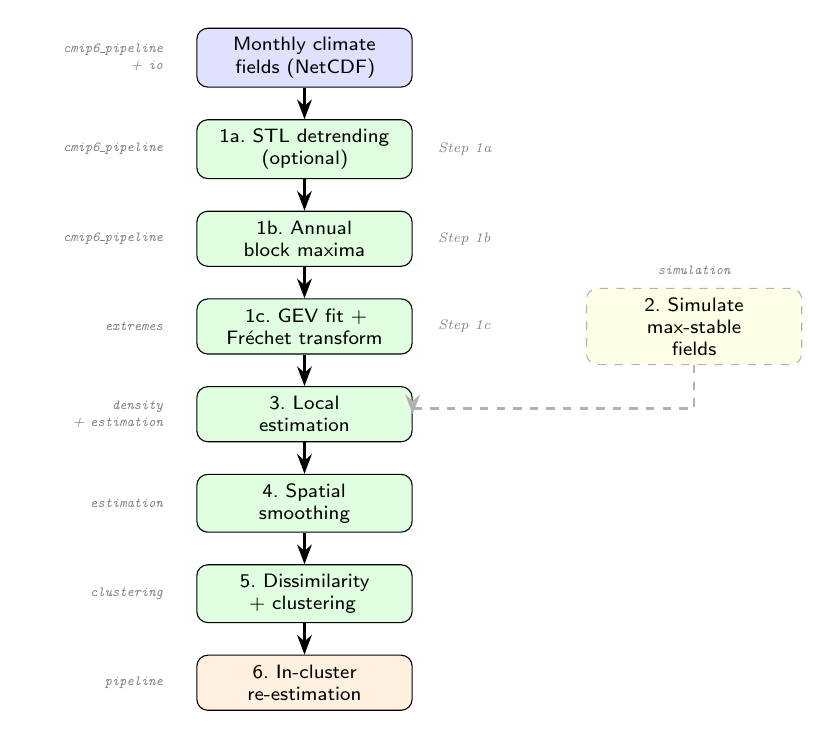
\begin{tikzpicture}[
  box/.style={draw, rounded corners=4pt, minimum width=2.6cm,
    minimum height=0.7cm, font=\sffamily\scriptsize,
    align=center, text width=2.5cm},
  data/.style={box, fill=blue!12},
  proc/.style={box, fill=green!12},
  outbox/.style={box, fill=orange!12},
  simbox/.style={box, fill=yellow!10, draw=gray!60, dashed},
  arr/.style={-{Stealth[length=2.5mm]}, thick},
  arrdashed/.style={-{Stealth[length=2.5mm]}, thick, dashed, gray!60},
  note/.style={font=\itshape\tiny, text=gray},
  node distance=0.4cm,
]

\node[data] (raw) {Monthly climate\\fields (NetCDF)};

\node[proc, below=of raw] (stl)
  {\rev{1a.\ STL detrending\\(optional)}};
\node[proc, below=of stl] (bm)
  {\rev{1b.\ Annual\\block maxima}};
\node[proc, below=of bm] (frech)
  {\rev{1c.\ GEV fit +\\Fr\'{e}chet transform}};
\node[proc, below=of frech] (mle)
  {3.\ Local\\estimation};
\node[proc, below=of mle] (smooth)
  {4.\ Spatial\\smoothing};
\node[proc, below=of smooth] (clust)
  {5.\ Dissimilarity\\+ clustering};
\node[outbox, below=of clust] (out)
  {6.\ In-cluster\\re-estimation};

\draw[arr] (raw) -- (stl);
\draw[arr] (stl) -- (bm);
\draw[arr] (bm) -- (frech);
\draw[arr] (frech) -- (mle);
\draw[arr] (mle) -- (smooth);
\draw[arr] (smooth) -- (clust);
\draw[arr] (clust) -- (out);

% Stage 2: simulation side-branch (optional validation path)
\node[simbox, right=2.2cm of frech] (sim)
  {\revt{2.\ Simulate\\max-stable\\fields}};
\node[note, above=0.05cm of sim, text width=2.5cm, align=center]
  {\texttt{simulation}};
\draw[arrdashed] (sim.south) -- ++(0,-0.55) -| (mle.east);

% Module names on the left
\node[note, left=0.3cm of raw, text width=1.6cm, align=right]
  {\texttt{cmip6\_pipeline}\\+ \texttt{io}};
\node[note, left=0.3cm of stl, text width=1.6cm, align=right]
  {\rev{\texttt{cmip6\_pipeline}}};
\node[note, left=0.3cm of bm, text width=1.6cm, align=right]
  {\rev{\texttt{cmip6\_pipeline}}};
\node[note, left=0.3cm of frech, text width=1.6cm, align=right]
  {\texttt{extremes}};
\node[note, left=0.3cm of mle, text width=1.6cm, align=right]
  {\texttt{density}\\+ \texttt{estimation}};
\node[note, left=0.3cm of smooth, text width=1.6cm, align=right]
  {\texttt{estimation}};
\node[note, left=0.3cm of clust, text width=1.6cm, align=right]
  {\texttt{clustering}};
\node[note, left=0.3cm of out, text width=1.6cm, align=right]
  {\texttt{pipeline}};

% Stage labels on the right
\node[note, right=0.2cm of stl] {Step 1a};
\node[note, right=0.2cm of bm] {Step 1b};
\node[note, right=0.2cm of frech] {Step 1c};

\end{tikzpicture}
\caption{\rev{Processing pipeline of \texttt{weatherisk}. Stage~1
  (a--c) is the preprocessing chain added for climate-model data;
  step~1a can be switched off;
  stages~3--6 implement the core statistical methodology of Contzen
  et al.~\cite{contzen2025}. Module names are shown on the left.\revt{ Stage~2
  (dashed box, right): \texttt{simulation.py} generates simulated
  max-stable fields on a regular 2-D grid with user-chosen dependence
  parameters and passes them to
  Stage~3 to check whether the pipeline gives back those known
  values.}}}
\label{fig:workflow}
\end{figure}

\subsection{Software functionalities}
\label{sec:functionalities}

Section~\ref{sec:architecture} describes the end-to-end workflow.
This subsection instead summarises the main software components and
their roles within the package.

\paragraph{Covariance modelling (\texttt{covariance})}
This module provides the correlation functions of the extremal-$t$
dependence model, which are anisotropic and either stationary or
non-stationary. It also converts correlations into extremal
coefficients and back.

\paragraph{Simulation (\texttt{simulation})}
The simulation module generates synthetic max-stable fields with
spatially varying anisotropy. These synthetic datasets are used for
method development, controlled validation experiments, and regression
tests against known parameter fields.

\paragraph{Preprocessing and extremes (\texttt{cmip6\_pipeline}, \texttt{netcdf}, \texttt{extremes})}
These components handle gridded climate-model input, including NetCDF
loading, optional STL detrending of monthly series (module \texttt{stl}), annual block-maxima
extraction, GEV fitting, and transformation to unit Fr\'{e}chet
margins. Together they provide the climate-data preprocessing chain
required before spatial dependence can be estimated.

\paragraph{Estimation (\texttt{density}, \texttt{estimation})}
These modules implement pairwise composite-likelihood estimation of
the local anisotropy parameters $(a,b,\gamma)$, the subsequent spatial
smoothing step, and the in-cluster re-estimation routines used after
clustering. They also contain the numerical safeguards needed for
stable optimisation on large grids.

\paragraph{Clustering (\texttt{clustering})}
This module provides the two regionalisation methods implemented in
\texttt{weatherisk}: LEC (Local Estimates Clustering), based on
ellipse-overlap dissimilarity, and EDC (Extremal Dependence
Clustering), based on madogram-derived extremal dependence. It also provides
the hierarchical clustering utilities that convert these
dissimilarities into region labels.

\paragraph{Scalability and execution (\texttt{scalable}, \texttt{cli})}
These components support large production runs through parallel
execution, checkpoint/restart handling, and command-line entry points
for the main workflows. They are designed to make the same code base
usable both for local experiments and for HPC-scale Figure~9
\revb{case-study analysis}.
The command-line entry point \texttt{weatherisk} has three
sub-commands: \texttt{validate} for the synthetic designs,
\texttt{cmip6} for the Figure~9 case study, and \texttt{maps} for
gridded observational data of the NOAA Climate Prediction Center
(CPC), for example:
\begin{lstlisting}[numbers=none]
$ weatherisk validate --params stripes \
    --resolution 10 --n-sim 20 --seed 42
\end{lstlisting}

\paragraph{Plotting and outputs (\texttt{plotting}, \texttt{map\_plotting})}
The plotting modules generate diagnostic figures, synthetic-study
visualisations, and the cluster maps of the CPC and CMIP6
workflows. They provide the final user-facing outputs of the
pipeline in addition to the saved numerical arrays.

\subsection{Computational performance}
\label{sec:performance}

Three parts of the pipeline dominate its cost: the local estimation,
which solves one multistart optimisation per grid cell; the
in-cluster re-estimation, which solves one optimisation over all
pairs of cells within distance $4\varepsilon$ in each cluster; and the
two dissimilarity matrices, whose $n(n-1)/2$ entries grow
quadratically with the number of cells~$n$.
\texttt{weatherisk} reduces these costs in four ways:

\begin{enumerate}
\item \textbf{Batch covariance.}
  In the simulation, all $n^2$ entries of the non-stationary
  covariance matrix are evaluated in one vectorised NumPy call, and
  the $2\times 2$ matrix inverses use the analytic closed-form formula.

\item \textbf{Vectorised ellipse overlap (LEC).}
  The quadratic form of each cell's ellipse is evaluated once on a
  fixed set of raster points. The overlap of two ellipses is the
  number of raster points inside both, divided by the number inside
  either, and is computed with boolean array operations for a block
  of rows of the dissimilarity matrix at a time (256 rows by default,
  64 in the CMIP6 pipeline) to bound memory use.

\item \textbf{Compiled pairwise distances (EDC).}
  The madogram distances between the rank vectors of all pairs of
  cells are computed by SciPy's compiled distance routines
  (\texttt{scipy.spatial.distance.\allowbreak{}pdist} in the CMIP6
  pipeline).

\item \textbf{Parallel estimation.}
  Per-cell optimisations, and in the last stage per-cluster
  optimisations, are distributed over worker processes with Python's
  \texttt{multiprocessing}; shared data is loaded once per worker.
\end{enumerate}

Table~\ref{tab:timing} reports measured run times at two scales.
The small benchmark runs the complete CMIP6 pipeline on a synthetic
$6\times6$ grid with 12~years of monthly data
(\texttt{scripts/run\_fig9\_benchmark.py --skip-plots}); it takes about 16\,s on a
laptop, about 80\% of which is local estimation. The full
AWI-ESM-1-1-LR T63 grid (18{,}432 cells, 156~years) was run on the
\revt{Alfred Wegener Institute (AWI)} \emph{albedo} HPC cluster with
64~worker processes, once with and once without STL detrending.
Local estimation took 11.9\,h and 11.8\,h of these runs, and both
dissimilarity matrices together about 5\,min. The in-cluster
re-estimation took the remaining 24\,h with STL detrending and
14\,h without. This stage assigns one worker to each cluster, so the
last clusters to finish (3{,}247 cells, the fourth-largest cluster,
in the STL run; 6{,}230 cells, the largest, in the run without
detrending) were each processed by a single worker while most of
the other cores were idle. The CPU utilisation averaged over the
whole job was therefore 35\% and 47\% of the 64 allocated cores.
Parallelising the re-estimation within a cluster is the most direct
way to shorten full-scale runs. SLURM scripts and setup are provided
under \texttt{hpc/}.

\begin{table}[!htbp]
\centering
\small
\begin{tabular}{lrr}
\toprule
 & \textbf{Synthetic $6\times6$} & \textbf{AWI-ESM-1-1-LR T63} \\
\midrule
Grid cells & 36 & 18{,}432 \\
Years & 12 & 156 \\
Hardware & Apple M4 laptop & albedo compute node \\
Worker processes & 4 & 64 \\
Wall time, STL detrending & 16.3\,s & 36.0\,h \\
Wall time, no detrending & --- & 26.0\,h \\
Share of local estimation & 80\% & 33\% / 46\% \\
Peak memory, all processes & 0.52\,GiB & 95\,GiB / 85\,GiB \\
\bottomrule
\end{tabular}
\caption{Measured run times and memory of the CMIP6 pipeline.
  Synthetic benchmark, without plotting: median of three repetitions (15.9, 16.3 and
  17.0\,s; local estimation 13.1\,s in the median run), commit
  \texttt{d28e36f}, peak resident memory summed over the process
  tree. T63 grid: one run per setting, given as STL / no detrending;
  the wall times cover stages 3--6, which were resumed from the
  checkpoint written after stage~1 (in the earlier job, STL detrending
  took 30\,s and the GEV step 9\,s), and the memory is the SLURM maximum of the resident
  memory summed over all processes, which counts shared pages more
  than once. The largest single process peaked at 36\,GiB and
  38\,GiB.}
\label{tab:timing}
\end{table}


%% ============================================================
\section{Illustrative examples}
\label{sec:examples}
%% ============================================================

We demonstrate \texttt{weatherisk} with \rev{two} examples: one on
synthetic data \rev{and one \revb{Python-based revisit of Figure~9 from Contzen}
et al.~\cite{contzen2025} on the AWI-ESM-1-1-LR climate model}.

\subsection{Example~1: Synthetic validation}
\label{sec:ex-synthetic}

In this example, we simulate extremal-$t$ max-stable data on a
51$\times$51 grid where the axis difference $b$ (Section~\ref{sec:architecture})
increases linearly from left to right, while $a = 2$ and $\gamma = 0$
are constant,
creating vertical ``stripe'' regions.  The pipeline should recover
these stripes from the simulated data alone.

\begin{lstlisting}[caption={Running the stripes validation.},
  label=lst:validate]
from weatherisk.pipeline import run_nonstationary_pipeline

# Preset "paper_stripes": 51x51 grid on [-5,5]^2,
# 250 replicates, true a = 2, gamma = 0, b(x, y) = (x + 5)/2
result = run_nonstationary_pipeline(
    "paper_stripes", seed=42, n_workers=8,
)
print(result["k_edc"], result["k_lec"])
\end{lstlisting}

\noindent Listing~\ref{lst:app-validate} in~\ref{app:code} runs the same
steps one function at a time.

Figure~\ref{fig:stripes} shows the result of this call run with
\texttt{n\_workers=32}, which took 8.4~hours of wall time.
Panel~(a) displays the EDC clusters ($k_{\text{edc}} = 7$),
panel~(b) the LEC clusters ($k_{\text{lec}} = 5$), and panel~(c)
the true field $b = (x+5)/2$, which rises from 0 on the left to 5
on the right. The in-cluster estimates of~$b$ of the seven EDC
clusters range from 0.31 to 3.73 and follow the left-to-right
trend, but several EDC boundaries run horizontally across the
domain, and no column of the grid lies within a single EDC cluster.
Four of the five LEC clusters are vertical bands, with in-cluster
estimates $b = 0.37$, 1.68, 3.42 and 4.60 from left to right; the
fifth is a cluster of 28~cells in the upper-right corner
($b = 5.07$). Of the 51~grid columns, 24 lie entirely within one
LEC cluster. If each cell is assigned the estimate of its cluster,
the mean absolute error with respect to the true~$b$ over the
2601~cells is 0.37 for LEC and 0.86 for EDC.
Contzen et al.~\cite{contzen2025} report the same contrast for this
design (their Figure~3): EDC clusters span a wide range of
$x$-coordinates, LEC clusters resemble vertical stripes, and LEC
leaves small clusters at the edge of the map, where fewer
neighbouring cells enter the local estimates. They obtain six
clusters with both methods. The counts need not agree, because
the Python package draws the 250 replicates with its own random
number generator, so the simulated data differ from theirs.
This controlled experiment shows that the Python
implementation recovers the known spatial structure.
Section~\ref{sec:validation} describes how each stage is compared
with the original R code.

\begin{figure}[!htbp]
\centering
\includegraphics[width=0.95\textwidth]{figures/fig3_stripes.png}
\caption{Synthetic validation on the ``stripes'' preset
  (seed~42, $k_{\text{edc}} = 7$, $k_{\text{lec}} = 5$).
  (a)~EDC clusters coloured by their estimated axis difference~$b$;
  (b)~LEC clusters coloured by their estimated~$b$;
  (c)~true field $b = (x+5)/2$, rising from 0 to~5.
  The LEC boundaries are mostly vertical, as in the true field,
  apart from a 28-cell cluster in the upper-right corner; several
  EDC boundaries run horizontally.}
\label{fig:stripes}
\end{figure}

\FloatBarrier

\rev{\subsection{Example~2: \revb{Revisiting the Figure~9 case study} --- AWI-ESM-1-1-LR
  global precipitation}
\label{sec:ex-fig9}}

\rev{To demonstrate the software on the same data used in the original
publication, we \revb{revisit the Figure~9 analysis} of Contzen et al.~\cite{contzen2025}.  The
experiment uses monthly precipitation from the AWI-ESM-1-1-LR
historical simulation (T63 grid, $192 \times 96$ cells, r1i1p1f1,
years 1850--2005) with the parameter settings listed in
Table~\ref{tab:fig9-params}, following Section~5 of~\cite{contzen2025}:}

\begin{table}[ht]
\centering
\begin{tabular}{ll}
\toprule
\textbf{Parameter} & \textbf{Value} \\
\midrule
Degrees of freedom $\nu$ & 5 \\
Covariance exponent $\alpha$ & 1 \\
Neighbour radius $\varepsilon$ & 5 (grid-point units) \\
Clustering quantile threshold & 30\textsuperscript{th} percentile \\
Model / experiment & AWI-ESM-1-1-LR / historical \\
Grid / resolution & T63 ($192 \times 96$) \\
Period & 1850--2005 (156~years) \\
\bottomrule
\end{tabular}
\caption{Parameter settings used for the Figure~9 \revb{case-study analysis},
  following Section~5 of Contzen et al.~\cite{contzen2025}. \revo{The degrees of
  freedom $\nu$ and the exponent $\alpha$ are parameters of the
  extremal-$t$ dependence model~\cite{opitz2013,contzen2025}: for a
  given correlation, a larger $\nu$ gives weaker extremal
  dependence, and $\alpha \in (0,\,2]$ is the exponent of the
  powered-exponential correlation function $\exp(-h^{\alpha})$ of
  the underlying Gaussian process, which sets how the correlation
  decays with the anisotropic distance~$h$.}}
\label{tab:fig9-params}
\end{table}

The pipeline (Section~\ref{sec:architecture}) was run twice on one
64-core node of the AWI \emph{albedo} HPC cluster with the SLURM
script \texttt{hpc/run\_fig9\_pyonly.slurm}: once with STL
detrending and once without it. The underlying invocations are:

\begin{lstlisting}[caption={\revb{Running the Figure~9 case study on HPC}.},
  label=lst:fig9, numbers=none]
$ python scripts/reproduce_fig9.py \
    --data-dir /path/to/AWI-ESM-1-1-LR/pr/ \
    --workers 64  --output-dir output/fig9_detrend
$ python scripts/reproduce_fig9.py \
    --data-dir /path/to/AWI-ESM-1-1-LR/pr/ \
    --workers 64  --output-dir output/fig9_nodetrend \
    --no-detrend
\end{lstlisting}

Figure~\ref{fig:fig9} shows both results, and
Table~\ref{tab:fig9-counts} compares the cluster counts with those
reported by Contzen et al.~\cite{contzen2025}. In both runs all
18{,}432 grid cells passed the screening of stage~1(c).

\begin{table}[ht]
\centering
\begin{tabular}{lcc}
\toprule
\textbf{Run} & \textbf{EDC ($k_{\text{edc}}$)} &
  \textbf{LEC ($k_{\text{lec}}$)} \\
\midrule
Contzen et al.~\cite{contzen2025} & 104 & 24 \\
\texttt{weatherisk}, no detrending & 104 & 23 \\
\texttt{weatherisk}, STL detrending & 142 & 14 \\
\bottomrule
\end{tabular}
\caption{Cluster counts for the Figure~9 case study: as reported by
  Contzen et al.~\cite{contzen2025}, and as obtained with
  \texttt{weatherisk} with and without STL detrending (30\% quantile
  threshold in all cases). Run times are given in
  Table~\ref{tab:timing}.}
\label{tab:fig9-counts}
\end{table}

The two runs differ only in the detrending step. Without
detrending, \texttt{weatherisk} gives the published
$k_{\text{edc}} = 104$, and $k_{\text{lec}} = 23$ against the
published 24. With STL detrending it gives $k_{\text{edc}} = 142$
and $k_{\text{lec}} = 14$. Contzen et al.~\cite{contzen2025} state
that the data were detrended with STL, but they do not report the
STL settings, and their R code, which we use as the reference in
Section~\ref{sec:validation}, covers the simulation study and does
not contain the preprocessing of the climate application. We
therefore cannot tell which
preprocessing produced the published counts, and we report both
runs.

The EDC count is the easier one to interpret, because the EDC chain
contains no numerical optimisation: the madogram depends only on the
ranks of the annual maxima, and the threshold rule and the
dendrogram are deterministic. We recomputed $k_{\text{edc}}$ on the
full grid for six STL variants: the setting above (periodic seasonal
component, robust fitting, trend removed); the same with the
seasonal component also removed; non-robust fitting; a seasonal
window \texttt{s.window} of 7 or of 13 instead of periodic; and the
period extended to 2014. They gave $k_{\text{edc}}$ between 138 and
146 with SciPy's merge order and between 137 and 147 with the merge
order of R's \texttt{hclust}. The annual maxima of the series without
detrending gave 104 with SciPy and 106 with R's merge order.
Differences of this size come from the order in which equal
dissimilarities are merged.
For the STL input, the R functions of Contzen et al.\ applied to the
same annual maxima give 140 instead of 142, and permuting the order
of tied entries gives values from 139 to 142. The count is also
sensitive to the quantile level: with STL detrending, a level of
about 0.34 instead of 0.30 would be needed to obtain 104 clusters.

The LEC count depends, in addition, on the local estimates
$(a_i, b_i, \gamma_i)$ and hence on the optimiser. On the synthetic
pipeline test data the Python optimiser attains R's likelihood, to
within $10^{-6}$, at every cell, and a higher one at 12 of the 25
cells (Section~\ref{sec:validation}). Where the
likelihood surface is flat, optima of equal likelihood can have
different parameters. An exact match of $k_{\text{lec}}$ with a
different optimiser is therefore not expected, and we do not
interpret the difference between 23 and 24.

Both runs used commit \texttt{7561a6e}. The only later change to the
package concerns the ranking of tied annual maxima in the madogram,
which now follows the R code; recomputing the EDC labels of both runs
from their stored GEV output with the current rule gives identical
labels.

During validation we also found an indexing error in the LEC code of
the original R implementation. In the function
\texttt{calc\_distance\_ellipses} (\texttt{r\_code/functions.R},
line 515 in the repository version used here\revt{; see
\url{https://github.com/wkchikach99-byte/weatherisk/blob/4cf18b2/r_code/functions.R\#L515}}),
the branch for an empty ellipse inside the loop over the grid-cell
indices \texttt{i} and \texttt{j} assigns \texttt{dist\_matrix[j] = 1}
instead of \texttt{dist\_matrix[i,j] <- 1}. Because R accepts a
single index into a matrix as a linear index, the function runs
without error, but the value is written to the wrong entry of the
dissimilarity matrix. \texttt{weatherisk} implements the intended
assignment; the corresponding validation test replays the R
behaviour so that the two codes can still be compared on identical
inputs.

\FloatBarrier
\begin{figure}[!htbp]
\centering
\includegraphics[width=\textwidth]{figures/fig9_pyonly_comparison.png}
\caption{The Figure~9 case study of Contzen
  et al.~\cite{contzen2025} recomputed with \texttt{weatherisk}: EDC clusters
  (left) and LEC clusters (right) of annual maxima of monthly
  AWI-ESM-1-1-LR historical precipitation (T63 grid, 1850--2005;
  $\nu = 5$, $\alpha = 1$, $\varepsilon = 5$, 30\% quantile
  threshold), computed without detrending (top row) and with STL
  detrending (bottom row). Colours only distinguish clusters within a
  panel and are reused when a panel has more clusters than colours.
  Contzen et al.\ report $k_{\text{edc}} = 104$ and
  $k_{\text{lec}} = 24$.}
\label{fig:fig9}
\end{figure}

\FloatBarrier


%% ============================================================
\rev{\section{Model validation}
\label{sec:validation}}
%% ============================================================


\rev{\texttt{weatherisk} contains no R code and starts no R process.
We therefore establish its correctness by comparison with outputs of
R that were computed once and are stored in the repository
(\texttt{tests/reference\_data/}), so that the comparison itself runs
without R. The stored outputs come from two sources: the R functions
of Contzen et al.~\cite{contzen2025}, evaluated on synthetic test
cases and on a simulated $10{\times}10$ field, and an R workflow that
we wrote for this purpose
(\texttt{tests/generate\_cmip6\_mini\_reference.R}). The workflow
combines these functions with R's \texttt{stl()} and runs the climate
pipeline, from detrending to clustering, on synthetic monthly
precipitation for a $5{\times}5$ grid and 20~years. The test suite has three levels
(Table~\ref{tab:validation}). The criterion at each level follows from
the kind of computation tested. Deterministic computations must agree
with R to rounding error. Numerical optimisation is judged by the
value of the objective it reaches, because two correct optimisers
started from different points need not return the same parameters.

\textbf{Level~1: individual functions (116 tests).}
Each R function that \texttt{weatherisk} translates is compared with
its Python counterpart on identical inputs. The functions include the
grid indexing, the covariance and extremal-coefficient functions, the
pairwise likelihood and its summands, the F-madogram, the
ellipse-overlap distance, the spatial smoothing and the LEC merge
heights. Deterministic functions must agree to absolute tolerances
between $10^{-14}$ and $10^{-10}$, depending on the function; in five
of these comparisons a relative tolerance of the same size is
allowed as well. On the simulated $10{\times}10$ field, the largest
difference observed for any of them is $1.4\times10^{-14}$. The STL module is compared with
R's \texttt{stl()} on 78~series in 14~configurations that differ in
length, period, seasonal window, polynomial degree, robustness and
jump settings, to a relative tolerance of $10^{-12}$. In one
configuration the series consist mostly of exact zeros. For these
series, a change of one unit in the
last place of the input moves R's own trend by $7\times10^{-10}$
(relative), so the trend is held to $10^{-9}$, the robustness weights
to $2\times10^{-5}$, and the set of zero weights must match exactly.
A further 22~tests cover the differences between the two languages
that had to be resolved during the translation: column-major versus
row-major storage, the parameter scaling of the optimiser, the
periodicity of the rotation angle~$\gamma$, the repetition of
optimisations that stop at a parameter bound, and the layout of the
in-cluster estimates. Four
tests check the treatment of tied values in the madogram ranks
against a transcription of the R loop. Two tests cover the local and
in-cluster optimisers and apply the likelihood criterion described
under Level~2. The EDC dendrogram is the one result that is not
held to rounding error. On the $10{\times}10$ field, many F-madogram
distances are tied, \texttt{hclust} and SciPy merge tied pairs in a
different order, and later merge heights differ by up to $0.0032$.
Two tests therefore check that each dendrogram is a valid
average-linkage run on the same distance matrix (every merge joins a
pair at the current minimum distance, to $10^{-14}$), and a third
that the threshold and the number of clusters equal R's exactly. Three looser
tests bound the sorted merge heights by $0.015$, allow the number of
clusters to differ by one, and require that at least 85\,\% of all
pairs of cells be assigned consistently (in the same cluster or in
different clusters); the measured agreement is 99.6\,\% (21 of
4{,}950 pairs differ).

\textbf{Level~2: the climate pipeline on synthetic data (16 tests).}
The synthetic monthly precipitation of the R workflow ($5{\times}5$
grid, 20~years, seasonal cycle, a weak trend and Gaussian noise) is
run through the Python pipeline, and the output of each stage is
compared with the stored output of the R workflow
(Table~\ref{tab:pipeline-parity}). Spatial smoothing and in-cluster
re-estimation are tested at Level~1. The GEV parameters are maximum
likelihood estimates computed by different optimisation routines in
the two languages, so they are compared to $10^{-3}$ rather than to
rounding error.
The local optimiser is judged by likelihood. At each of the
25~cells, both parameter vectors are evaluated with the same
likelihood function, and the pairwise negative log-likelihood,
summed over all neighbour pairs of the cell, may exceed its value at
R's optimum by at most~0.03. Equal parameters are not a meaningful
target here. Each cell has 20~annual maxima, and when $a$ is at its
lower bound the likelihood is nearly flat in $b$ and $\gamma$, so
very different parameter vectors reach the same likelihood, and the
one R reports depends on its random starting values. In the
measurement, the Python value is lower than R's at 12~cells (by up
to $0.27$), equal within $10^{-6}$ at the other 13, and never higher
by more than $7.3\times10^{-7}$.
The ellipse-overlap distance is compared with R's behaviour
reproduced exactly, including the indexing error discussed in
Section~\ref{sec:ex-fig9}, so that the test measures the translation
alone. LEC clustering is tested apart from the optimiser: Python
receives R's own smoothed local estimates and must reproduce R's
threshold and $k$. EDC clustering must reproduce R's threshold and
$k$ ($k_{\text{edc}}=7$). The resulting partitions are also identical
(adjusted Rand index~1), a property we checked but that the test does
not assert.
Table~\ref{tab:fig9-counts} reports the cluster counts at full scale.

\textbf{Level~3: structure and regression (103 tests).}
These tests do not compare with R. They cover checkpointing and
resumption (7~tests), equality of serial and parallel results and
of fast and reference implementations of the same computation (5), a static check that the package source contains no R calls
(2), the synthetic designs of Contzen et al.~\cite{contzen2025}
(parameter presets, the quantile threshold rule, non-stationary
fields and the Figure~3 workflow; 39), and the remaining components
and known regressions (50).

\begin{table}[!htbp]
\centering
\small
\setlength{\tabcolsep}{5pt}
\begin{tabularx}{\textwidth}{>{\raggedright\arraybackslash}p{5.6cm}c>{\raggedright\arraybackslash}X}
\toprule
\textbf{Level} & \textbf{Tests} & \textbf{Criterion} \\
\midrule
1.~Individual functions & 116 &
  absolute $10^{-14}$ to $10^{-10}$ for deterministic functions;
  likelihood criterion for the two optimisers \\
2.~Pipeline, synthetic data & 16 &
  per stage (Table~\ref{tab:pipeline-parity}) \\
3.~Structure and regression & 103 & per test \\
\quad checkpoint and resume & 7 & correct resume \\
\quad serial/parallel, fast/reference & 5 & equal to $10^{-10}$ or better \\
\quad no R calls in the package & 2 & none found \\
\quad synthetic designs of~\cite{contzen2025} & 39 & per test \\
\quad other components & 50 & per test \\
\midrule
\textbf{Total} & \textbf{235} & \\
\bottomrule
\end{tabularx}
\caption{Summary of the automated test suite. With R removed from the
  search path, all 235~tests pass in about 2\,min on an Apple M4
  laptop. Continuous integration skips the one end-to-end test that is
  marked as slow.}
\label{tab:validation}
\end{table}

\begin{table}[!htbp]
\centering
\small
\setlength{\tabcolsep}{4pt}
\begin{tabularx}{\textwidth}{>{\raggedright\arraybackslash}p{3.3cm}c>{\raggedright\arraybackslash}X>{\raggedright\arraybackslash}p{3.0cm}}
\toprule
\textbf{Pipeline stage} & \textbf{Tests} &
  \textbf{Criterion} & \textbf{Largest deviation} \\
\midrule
STL detrending & 3 &
  absolute difference $\leq 10^{-13}\max|x|$\textsuperscript{a} & \mbox{$2.3{\times}10^{-14}\max|x|$} \\
Annual maxima & 1 &
  relative error $\leq 10^{-12}$ & $2.0\times10^{-14}$ \\
GEV fit and Fr\'{e}chet transform & 1 &
  GEV parameters: absolute $\leq 10^{-3}$; Fr\'{e}chet margins:
  relative $\leq 2\times10^{-3}$ & $4.2\times10^{-4}$;
  $9.6\times10^{-4}$ \\
Local estimation & 2 &
  $\mathrm{NLL}_{\text{Python}} \leq \mathrm{NLL}_{\text{R}} + 0.03$
  at every cell\textsuperscript{b} & $+7.3\times10^{-7}$ \\
Ellipse-overlap distance & 1 &
  relative error $\leq 5\times10^{-15}$ & $1.9\times10^{-15}$ \\
LEC clustering & 1 &
  threshold within $10^{-14}$, $k$ equal, on R's smoothed estimates
  & $k$ equal \\
EDC madogram & 3 &
  absolute difference $\leq 10^{-10}$\textsuperscript{c} & $5\times10^{-16}$ \\
EDC clustering & 3 &
  threshold within $10^{-12}$, $k$ equal\textsuperscript{c} & $k$ equal \\
Configuration defaults & 1 &
  identical in both pipelines & -- \\
\midrule
\textbf{Total} & \textbf{16} & & \\
\bottomrule
\end{tabularx}
\caption{Stage-by-stage comparison of the Python pipeline with stored
  outputs of the R workflow on synthetic monthly precipitation
  ($5{\times}5$ grid, 20~years). $x$ denotes the monthly precipitation
  series; NLL is the pairwise negative log-likelihood summed over the
  neighbour pairs of a cell. The criterion and the last column refer
  to the comparisons with R; the last column gives the largest
  deviation measured in the test run. Not every test in a row
  compares with R:
  \textsuperscript{a}one test checks that the detrending is closer to
  STL than to a running mean;
  \textsuperscript{b}one test checks that the pipeline and the
  function-level entry point of the local optimiser return the same
  estimates;
  \textsuperscript{c}two madogram tests and one clustering test
  compare the pipeline's EDC functions with the function-level
  implementation on the $10{\times}10$ field of Level~1.}
\label{tab:pipeline-parity}
\end{table}}

\FloatBarrier

%% ============================================================
\section{Impact}
\label{sec:impact}
%% ============================================================

\revg{The core output of \texttt{weatherisk} is a partition of the
grid into spatially coherent regions, far fewer than the grid cells, each characterised by a common extremal
dependence structure. Working with these regions rather than
thousands of individual grid cells makes the analysis tractable and
raises concrete applied questions: which areas share a common
extreme-precipitation hazard, how do hazard boundaries shift across
climate states, and where should spatial risk aggregation be drawn
in insurance or infrastructure planning?}

\revo{\texttt{weatherisk} makes the method of Contzen
et al.~\cite{contzen2025} available as a Python library. The complete workflow, from monthly
model output to cluster maps, is contained in one package that is
installed with \texttt{pip install} and does not need R.}

\rev{\paragraph{Reproducibility and correctness}
The test suite of Section~\ref{sec:validation} lets a user check
an installation against stored outputs of R without installing R. It
compares individual functions and, on synthetic data, the stages of
the climate pipeline with these outputs, and it checks
checkpointing, parallel execution and the synthetic designs of the
original study. All 235~tests pass with R removed from the search
path.
Continuous integration runs the tests not marked as slow on every
push and pull request to the main branch, under Python~3.10 and~3.11.}

\paragraph{Computational efficiency}
Section~\ref{sec:performance} describes the vectorisation and
parallelisation used. The synthetic $6{\times}6$ benchmark runs in about 16\,s on a
laptop, and the full AWI-ESM-1-1-LR T63 grid (18{,}432 cells,
156~years) in 26--36\,h on 64~cores of the AWI \emph{albedo} HPC
cluster (Table~\ref{tab:timing}). The pipeline writes a checkpoint
after each step, and after each cluster within the final step, so an
interrupted run resumes from the last completed unit of work.

\revg{The pairwise dissimilarity matrix has $n^2$ entries for $n$
grid cells, and this quadratic cost remains the main limit on grid
size. Vectorisation and parallelisation reduce the constant factor
but not the growth rate. Kilometre-scale models would need sparse
approximations or graph-based clustering.}

\revg{\revo{One methodological limitation of} the present framework is
its reliance on block maxima\revr{: only the largest value per year
and grid cell is used, so further extremes within the same year do
not enter the analysis}.
This choice is justified within extreme value theory and matches
max-stable modelling. Future work could explore peaks-over-threshold
(POT) extensions in a spatial setting~\cite{davison2012}, which use
more of the data within the same theoretical framework.}

\paragraph{New research directions}
The Python API and the command-line interface can be applied to
other variables (for example wind speed or sea-level pressure) and
other datasets (for example ERA5 or CMIP6 projections). These
applications are not tested in this paper.

\paragraph{Education}
The step-by-step pipeline, the test suite and the code examples in~\ref{app:code} can be used to teach spatial extreme-value analysis.
The repository includes a Jupyter notebook
(\texttt{notebooks/\allowbreak weatherisk\_quickstart.ipynb}) that runs the
lightweight synthetic check \texttt{run\_pipeline}. It simulates a
max-stable field, computes the ellipse-overlap dissimilarity and
clusters the grid cells. It does not run local estimation.

%% ============================================================
\section{Conclusions}
\label{sec:conclusions}
%% ============================================================

\revo{We have presented \texttt{weatherisk}, a Python package that
implements the complete pipeline for spatial clustering of climate
extremes via max-stable processes. The package covers the full
preprocessing chain---optional STL detrending, annual block-maxima extraction,
GEV fitting, and Fr\'{e}chet transformation---followed by local
composite-likelihood estimation of anisotropy parameters and
regionalisation using Local Estimates Clustering (LEC) or Extremal
Dependence Clustering (EDC)~\cite{contzen2025}. The whole workflow is
contained in a single tested Python library that is installed with
\texttt{pip install} and runs without R.}

\revg{The software is compared with stored outputs of R function by
function and, on synthetic data, stage by stage through the climate
pipeline; a third group of tests covers structure and known
regressions. None of the 235~tests calls R. Deterministic functions
agree with R to absolute tolerances between $10^{-14}$ and
$10^{-10}$, and the STL decomposition to a relative tolerance of
$10^{-12}$ (looser for one series that consists mostly of zeros).
The exception is the EDC dendrogram on a simulated field with many
tied distances, where R and SciPy merge tied pairs in a different
order; the threshold and the number of clusters still agree exactly.
On the synthetic pipeline data, the negative log pairwise likelihood
reached by the local optimiser must not exceed R's by more than~0.03
at any cell; measured, it is lower at 12 of 25 cells and never higher
by more than $10^{-6}$. Parameter values are not compared, because
the likelihood of these data is nearly flat in $b$ and $\gamma$
where $a$ is at its lower bound. EDC, and LEC applied to R's
smoothed local estimates, reproduce R's threshold and number of
clusters on these data. The full Figure~9
\revb{case study} on the AWI-ESM-1-1-LR T63 grid ran in 26 to 36~hours
on 64~cores. Without detrending it reproduces the published EDC count
of 104 (R's \texttt{hclust} gives 106 on the same distances, because
it merges tied pairs in a different order) and gives 23 LEC clusters
against 24; the dependence of the
counts on detrending (Section~\ref{sec:ex-fig9}) shows that the
preprocessing has to be reported with the clustering.}

\revg{The clusters condense a large climate field into a small set of
regions in which extremes co-occur. Such regions are the spatial units
needed for risk aggregation in reinsurance, infrastructure planning,
and climate services. The current design has two limits. The
block-maxima approach uses only one value per grid cell per year, so
further extremes within the same year are not used. The number of
pairwise comparisons grows quadratically with the number of grid
cells, so kilometre-scale grids are impractical with the current
algorithm.}

\revo{Each limit suggests further work. Peaks-over-threshold
extensions in a spatial setting~\cite{davison2012} would use more of
the data within the same theoretical framework, and sparse or
graph-based dissimilarity approximations would reduce the quadratic
scaling. GPU computation with CuPy~\cite{okuta2017} or just-in-time
compilation with Numba~\cite{lam2015} could reduce the cost per pair.
Neither changes the quadratic number of pairs or the statistical
method.}

\revg{\paragraph{Outlook: Digital Earth System Twins}
High-resolution digital replicas of the Earth system, such as those
being developed in the European Destination Earth
initiative~\cite{bauer2021}, will require automated analysis tools
that operate at the same scale and cadence.
Spatial clustering of extremes could be one step in such a pipeline,
converting per-cell dependence estimates into a small set of
homogeneous regions that can be passed to impact models.
Future extensions would require incremental cluster updating, linkage
to socioeconomic exposure databases, and objective criteria for
detecting structural regime shifts.}

\revg{\texttt{weatherisk} is available under the MIT licence.}

%% ============================================================
%% APPENDIX
%% ============================================================
\appendix

\section{Key code examples}
\label{app:code}

\subsection{Synthetic validation}

\begin{lstlisting}[caption={Complete synthetic validation
  workflow.}, label=lst:app-validate]
import numpy as np
from scipy.cluster.hierarchy import fcluster
from weatherisk.parameters import get_preset
from weatherisk.grid import Grid
from weatherisk.simulation import sim_expt_2d_nonstat
from weatherisk.density import run_local_mle_parallel
from weatherisk.estimation import (
    smooth_local_estimates,
    calc_estimates_in_clusters,
)
from weatherisk.clustering import (
    calc_distance_ellipses,
    c_extrcoeff_matrix,
    clustering,
    quantile_threshold,
    cluster_number_threshold_method,
)
from weatherisk.plotting import plot_cluster_comparison

# 1. Preset, grid and true parameter fields
p = get_preset("paper_stripes")
grid = Grid(x_range=(-5, 5), y_range=(-5, 5),
            resolution=p.resolution)
a, b, g = (f(grid.X, grid.Y)
           for f in (p.a_func, p.b_func, p.g_func))

# 2. Simulate the non-stationary max-stable process
data = sim_expt_2d_nonstat(
    grid, p.df, p.alpha, a, b, g,
    n_sim=p.n_sim, rng=np.random.default_rng(42),
)

# 3. Local composite-likelihood MLE, then smoothing
loc = run_local_mle_parallel(
    data, grid, p.df, p.alpha,
    abstand=p.locest_abst, ensemble=p.locest_ensemble,
    n_workers=8,
)
sm = smooth_local_estimates(loc, p.smoothing_dist, grid)

# 4. Hierarchical clustering; k from the 30% quantile rule
def cut(dm, q=0.30):
    hc = clustering(dm)
    k = cluster_number_threshold_method(
        hc, quantile_threshold(dm, q))
    return fcluster(hc, t=max(2, k), criterion="maxclust")

labels_lec = cut(calc_distance_ellipses(sm, res=21))      # LEC
labels_edc = cut(c_extrcoeff_matrix(data, madogram=True))  # EDC

# 5. Re-estimate within clusters and plot (cf. Figure 2)
in_lec = calc_estimates_in_clusters(data, labels_lec,
                                    p.df, p.alpha, grid)
in_edc = calc_estimates_in_clusters(data, labels_edc,
                                    p.df, p.alpha, grid)
plot_cluster_comparison(
    grid, labels_edc, labels_lec, in_edc, in_lec, b,
    param_index=1, vmin=0, vmax=5, label="$b$",
    filename="stripes_clusters.png",
)
\end{lstlisting}

\rev{\subsection{CMIP6 Figure~9 \revb{case-study workflow}}}

\begin{lstlisting}[caption={\revb{Running the Figure~9 case study} on HPC or
  locally.}, label=lst:app-fig9]
# On HPC (albedo SLURM cluster):
$ sbatch hpc/run_fig9_pyonly.slurm

# Or locally (requires CMIP6 data):
$ python scripts/reproduce_fig9.py \
    --data-dir /path/to/AWI-ESM-1-1-LR/pr/ \
    --workers 8

# Programmatic access:
from weatherisk.cmip6_pipeline import (
    run_cmip6_pipeline,
    CMIP6Config,
)
cfg = CMIP6Config()  # paper defaults
results = run_cmip6_pipeline(cfg)
# results contains: labels_lec, labels_edc,
#   k_lec, k_edc, smoothed, frechet, ...
\end{lstlisting}

%% ============================================================
\section*{CRediT authorship contribution statement}
%% ============================================================
\textbf{Widad Kchikach:} Methodology, Software, Validation,
Investigation, Visualization, Writing -- original draft.
\textbf{Thorsten Dickhaus:} Conceptualization, Supervision,
Writing -- review \& editing.
\textbf{Gerrit Lohmann:} Conceptualization, Supervision,
Writing -- review \& editing.

%% ============================================================
\section*{\revn{Declaration of Competing Interests}}
%% ============================================================

\revn{The authors declare that they have no known competing financial
interests or personal relationships that could have appeared to
influence the work reported in this paper.}

%% ============================================================
\section*{Data availability}
%% ============================================================
The AWI-ESM-1-1-LR historical simulation used in
Section~\ref{sec:ex-fig9} is publicly available from the Earth
System Grid Federation~\cite{danek2020}. The synthetic data of
Section~\ref{sec:ex-synthetic} are generated by the package from the
seed given there.

%% ============================================================
\section*{Declaration of generative AI and AI-assisted technologies in the manuscript preparation process}
%% ============================================================
% AUTHOR CHECK: state the tools you used and what for; the wording after the first sentence is Elsevier's required text.
During the preparation of this work the authors used Claude
(Anthropic) in order to assist with writing and testing code and
with editing the manuscript text. After using this tool, the
authors reviewed and edited the content as needed and take full
responsibility for the content of the published article.

%% ============================================================
\section*{Acknowledgements}
%% ============================================================
The authors thank the Alfred Wegener Institute Helmholtz Centre for
Polar and Marine Research (AWI) for access to the \emph{albedo}
computing cluster, on which the Figure~9 case-study pipeline was
executed. We thank J.~Contzen for the original R implementation of
the methods, on which \texttt{weatherisk} is based.

\paragraph*{Funding}
W.~Kchikach is supported by the MarDATA Helmholtz School for Marine
Data Science (grant no.\ HIDSS-0005). G.~Lohmann acknowledges
support from the ERC Synergy Grant ``i2B'' (grant no.\ 101118519).


%% ============================================================
%% REFERENCES
%% ============================================================
\begin{thebibliography}{00}

\bibitem{davison2012}
A.C.~Davison, S.A.~Padoan, M.~Ribatet,
Statistical modeling of spatial extremes,
Stat.\ Sci.\ 27\,(2) (2012) 161--186.

\bibitem{dehaan2006}
L.~de~Haan, A.~Ferreira,
Extreme Value Theory: An Introduction,
Springer, New York, 2006.

\bibitem{padoan2010}
S.A.~Padoan, M.~Ribatet, S.A.~Sisson,
Likelihood-based inference for max-stable processes,
J.\ Am.\ Stat.\ Assoc.\ 105\,(489) (2010) 263--277.

\bibitem{contzen2025}
\rev{J.~Contzen, T.~Dickhaus, G.~Lohmann,
Regionalization approaches for the spatial analysis of extremal
dependence,
Extremes 28 (2025) 713--737.
\url{https://doi.org/10.1007/s10687-025-00519-2}}

\bibitem{pyextremes}
G.~Bocharov,
pyextremes: Extreme value analysis in Python,
\url{https://github.com/georgebv/pyextremes}, 2023.

\bibitem{spatialextremes}
M.~Ribatet,
SpatialExtremes: Modelling Spatial Extremes,
R package, \url{https://CRAN.R-project.org/package=SpatialExtremes}, 2023.

\bibitem{cleveland1990}
\rev{R.B.~Cleveland, W.S.~Cleveland, J.E.~McRae, I.~Terpenning,
STL: A seasonal-trend decomposition procedure based on loess,
J.\ Official Stat.\ 6\,(1) (1990) 3--73.}

\bibitem{schlather2002}
M.~Schlather,
Models for stationary max-stable random fields,
Extremes 5\,(1) (2002) 33--44.

\bibitem{opitz2013}
T.~Opitz,
Extremal $t$ processes: Elliptical domain of attraction and a
spectral representation,
J.\ Multivariate Anal.\ 122 (2013) 409--413.

\bibitem{cooley2006}
D.~Cooley, P.~Naveau, P.~Poncet,
Variograms for spatial max-stable random fields,
in: P.~Bertail, P.~Soulier, P.~Doukhan (Eds.),
Dependence in Probability and Statistics,
Springer, 2006, pp.~373--390.

\bibitem{saunders2021}
K.~Saunders, A.G.~Stephenson, D.J.~Karoly,
A regionalisation approach for rainfall based on extremal dependence,
Extremes 24\,(2) (2021) 215--240.

\bibitem{okuta2017}
R.~Okuta, Y.~Unno, D.~Nishino, S.~Hido, C.~Loomis,
CuPy: A NumPy-compatible library for NVIDIA GPU calculations,
in: Proceedings of Workshop on Machine Learning Systems,
2017.

\bibitem{lam2015}
S.K.~Lam, A.~Pitrou, S.~Seibert,
Numba: A LLVM-based Python JIT compiler,
in: Proceedings of the Second Workshop on the LLVM Compiler
Infrastructure in HPC,
2015, pp.~1--6.

\bibitem{bauer2021}
P.~Bauer, B.~Stevens, W.~Hazeleger,
A digital twin of Earth for the green transition,
Nat.\ Clim.\ Change 11\,(2) (2021) 80--83.

\bibitem{danek2020}
[dataset] C.~Danek, X.~Shi, C.~Stepanek, H.~Yang, D.~Barbi,
J.~Hegewald, et~al.,
AWI AWI-ESM1.1LR model output prepared for CMIP6 CMIP historical,
version 20200212, Earth System Grid Federation (2020),
\url{https://doi.org/10.22033/ESGF/CMIP6.9328}.

\end{thebibliography}

\end{document}
